\section{Mage-VL}
\label{sec:magevl}

Building upon the codec-native visual encoder introduced in \cref{sec:magevit}, we develop \magevl, a unified multimodal model for image understanding, offline video reasoning, and proactive interaction over continuous video streams. The same model supports static images, videos of varying durations, event-triggered commentary, and conventional user-initiated question answering.

\Cref{sec:magevl_arch} presents the unified architecture across image, offline-video, and streaming modes. \Cref{sec:magevl_data} describes the image, video, and streaming supervision, while \cref{sec:magevl_training} details the progressive five-stage training curriculum.

\begin{figure*}[t]
    \centering
    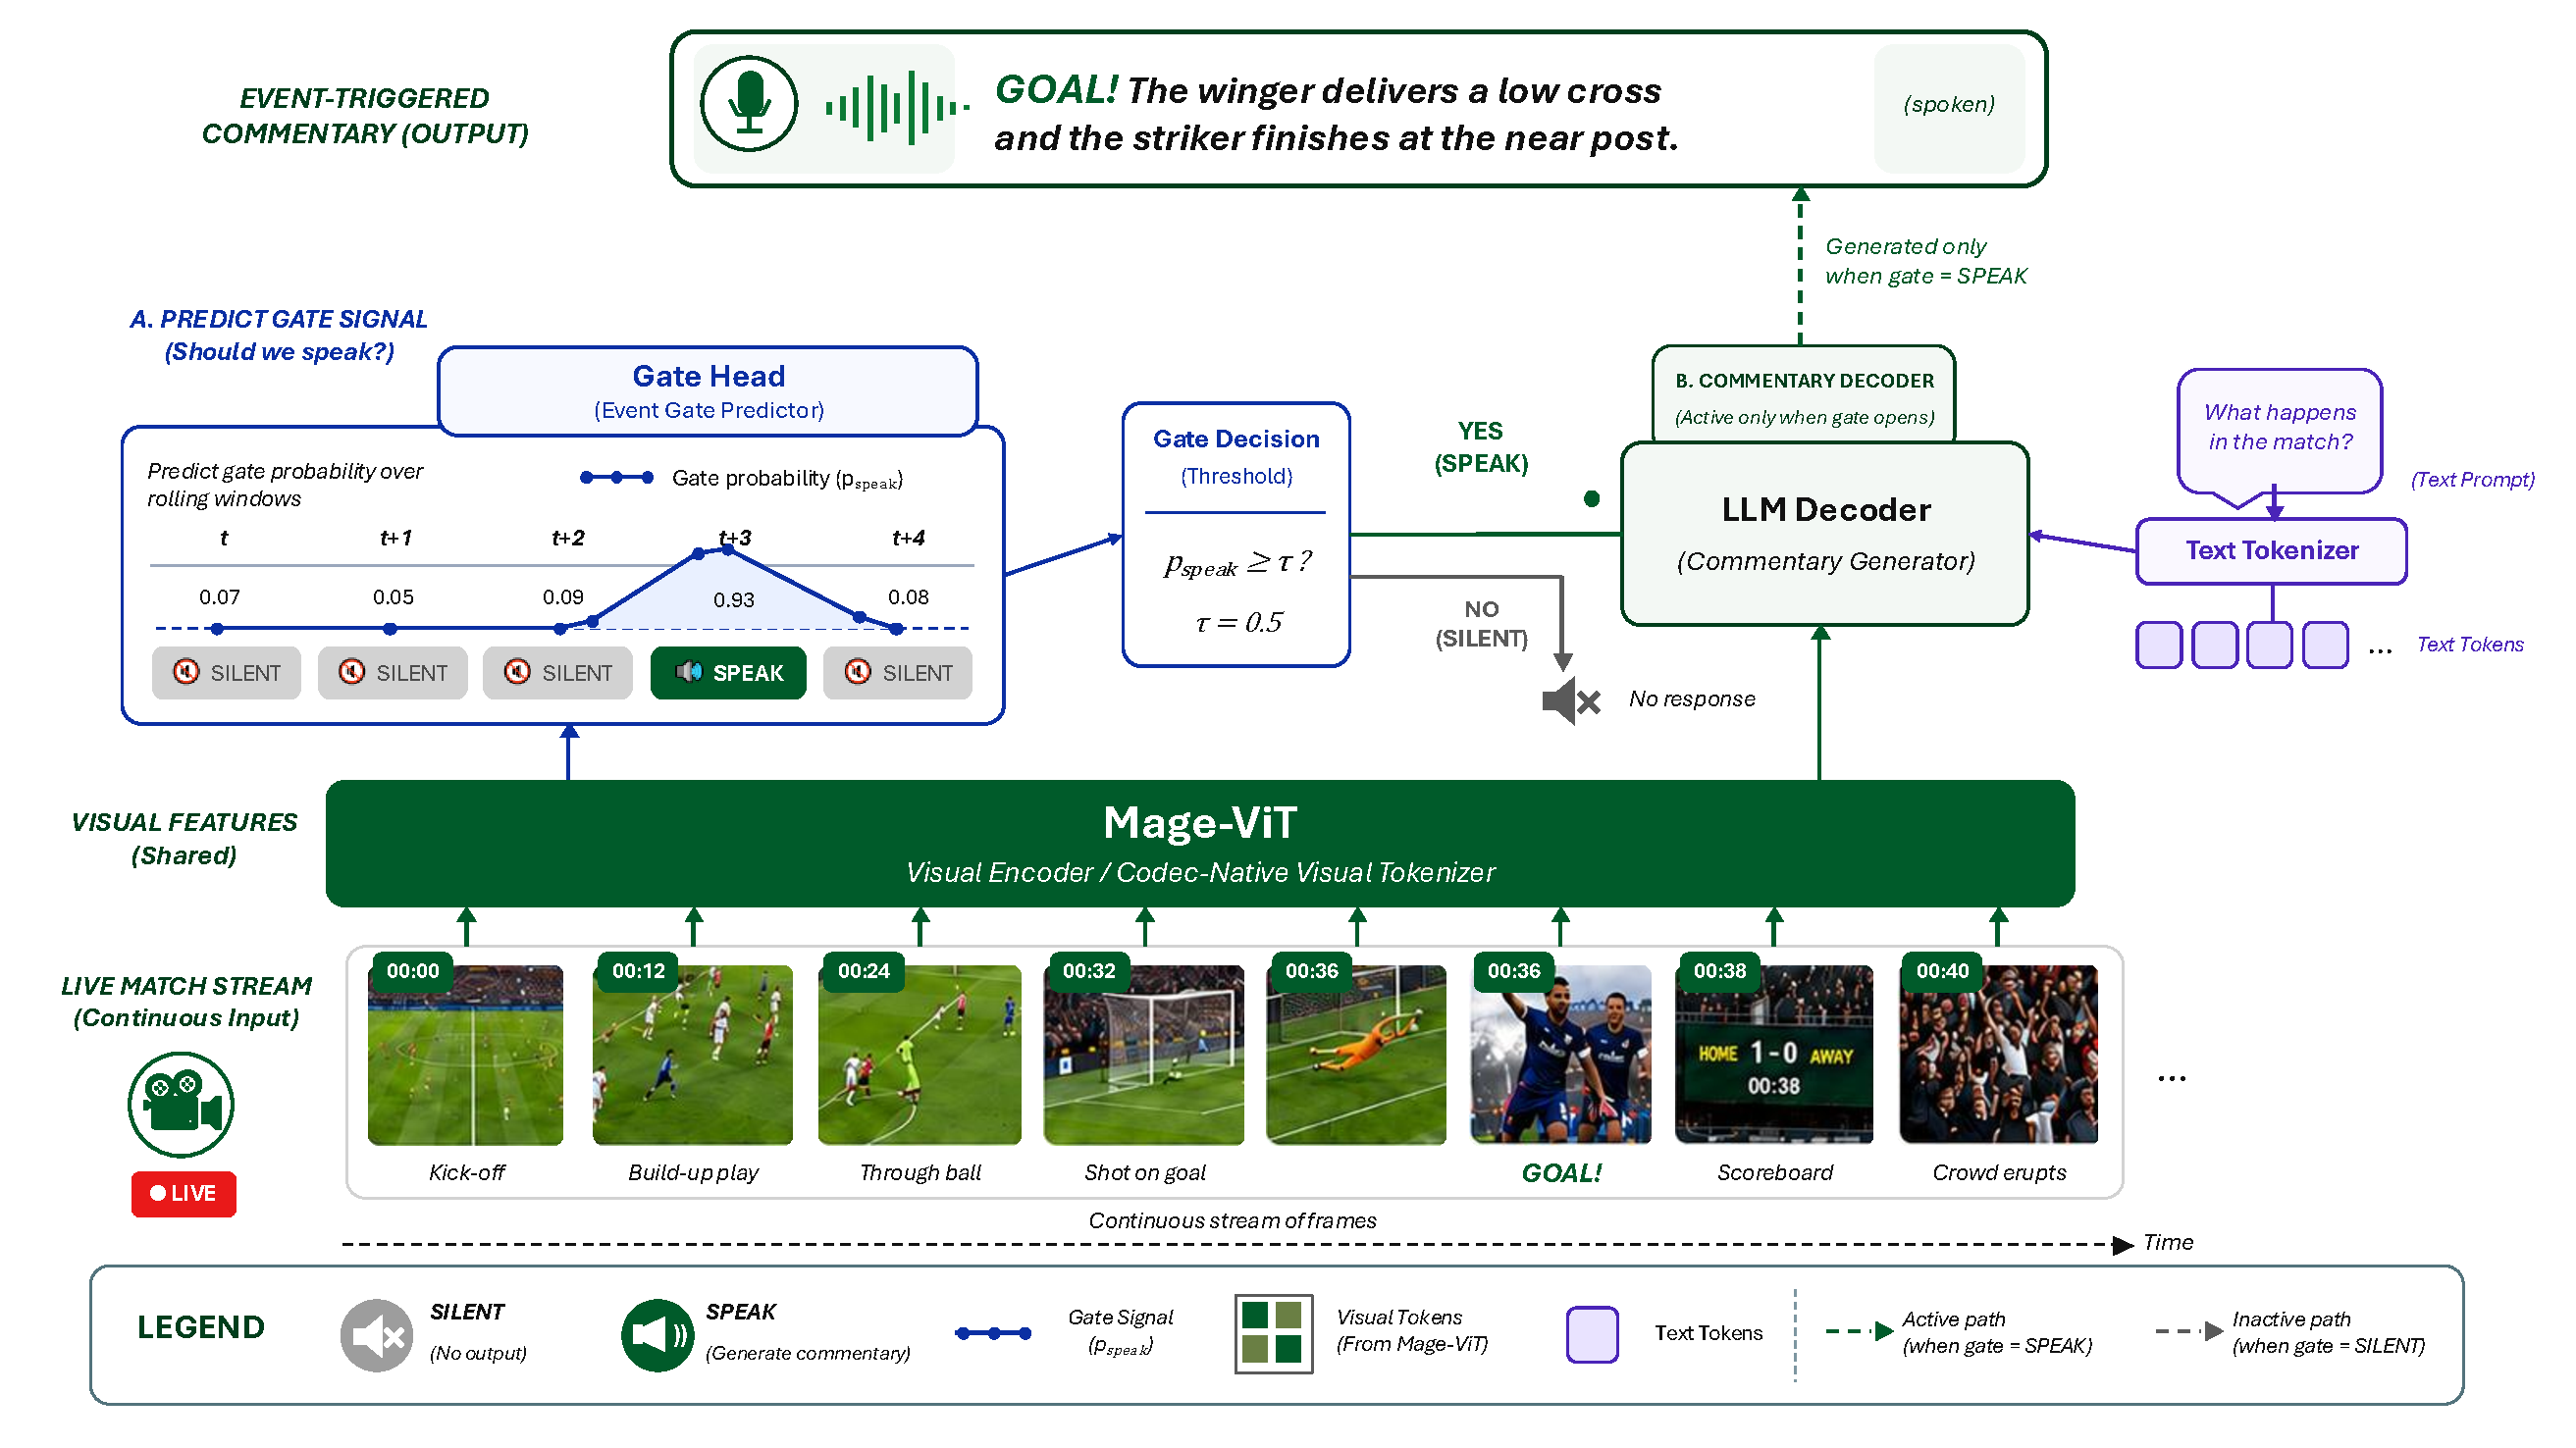
\includegraphics[width=\textwidth]{figures/FrameworkV5.pdf}
    \caption{\textbf{Proactive streaming framework of \magevl.} \magevit incrementally encodes a continuous video stream into codec-native visual features shared by the event gate and causal language decoder. The gate evaluates each rolling visual window and predicts whether the current prefix contains a response-worthy event. The model remains silent when the gate is closed; when it opens, the decoder generates an event-conditioned response from the recent visual context and the given text prompt.}
    \label{fig:magevl_framework}
\end{figure*}

\subsection{Unified Architecture}
\label{sec:magevl_arch}

\paragraph{Codec-native visual encoder.}
\magevl uses \magevit as its shared visual encoder across image, video, and streaming inputs. A still image is represented as a single spatial token sequence. For video, \magevit produces temporally ordered codec-token windows composed of densely encoded anchor-frame patches and sparsely selected predicted-frame patches. Anchor frames preserve complete scene context, whereas predicted frames retain only patches associated with motion or visual changes. This codec-native representation avoids repeated computation over temporally static regions while preserving fine-grained spatial and temporal information. The resulting visual features are passed to the vision-language projector and causal language decoder.

\paragraph{Vision-language projector.}
A lightweight two-layer MLP maps \magevit features into the token-embedding space of the language model. Because \magevit applies shared 3D rotary positional encoding over the original spatio-temporal grid, retained tokens preserve their original spatial and temporal coordinates after codec-driven sparse selection.

\paragraph{Causal language decoder.}
The language backbone is initialized from Qwen3-4B-Instruct-2507~\cite{qwen3}. Projected visual tokens and text tokens are processed by the same causal decoder. For images, visual tokens form a single block preceding the text instruction. For videos, codec-token windows are concatenated in temporal order. This unified interface allows \magevl to process images, short videos, long videos, and ultra-long videos without modifying the language backbone or introducing modality-specific decoders.

\paragraph{Proactive streaming mechanism.}
As illustrated in Fig.~\ref{fig:magevl_framework}, a lightweight cognition gate continuously evaluates the visual features of incoming codec windows. Given the current streaming representation $\mathbf{h}_t$, the gate predicts $p_{\mathrm{speak}}=g(\mathbf{h}_t)$ and triggers generation when $p_{\mathrm{speak}}\geq\tau$, where $\tau$ is a fixed inference threshold. Background segments and non-response-worthy moments keep the gate closed, whereas relevant events activate language generation.

During streaming inference, newly arrived codec windows are incrementally processed by the perception pathway. The cognition gate evaluates the accumulated streaming memory, while response generation uses a local sliding window containing the most recent codec-token segments. A text query may be inserted at any time, whereas proactive responses are controlled by the cognition gate. This design supports continuous perception, event-triggered commentary, and user-initiated interaction within the same model.


\subsection{Data Construction}
\label{sec:magevl_data}
Our training corpus contains approximately \textbf{350M image--caption pairs}, \textbf{54M image-instruction samples}, \textbf{7.95M unique video--caption samples}, and \textbf{3.35M streaming samples}. Caption data establish broad visual-language and temporal grounding, whereas instruction data provide task-oriented reasoning, response formatting, and grounding behavior. The streaming corpus further supervises response timing over causal video prefixes. During video training, selected image-instruction samples are interleaved with video data to preserve static-image understanding and general instruction-following capabilities.
% Data audit against the training manifests and packed tar files (2026-07-20):
% the reported corpus-level totals are broadly consistent with the underlying data.
% We scanned every available tar.idx and summed sample_count from every packed JSON.
% Stage 1: 4,823,785 packed records = 83,943,932 image--text samples; the shared
% Stage-1/1.5 mixed set has 3,686,525 packed records = 24,540,000 source samples.
% The Stage-1.5 image corpus is nominally 270M but was no longer available to scan;
% 83,943,932 + 270M is approximately 354M image captions before rounding. Stage 2
% contains 54,926,464 image-instruction samples and 3,393,358 caption-video samples.
% Stage 3 packed subsets: 157,681 = 9,961,834 (10M mixture), 189,380 = 2,065,231
% (LLaVA-Video mixture), 6,823 = 19,466 (TimeLens), and 2,307 = 113,707 (MIMO).
% Stage 4 packed subsets: 709,729 = 43,919,717 (image SFT), 76,143 = 4,607,927
% (spatial/GUI), 15,350 = 266,158 (VSI), 4,005 = 100,022 (OCR),
% 2,648 = 97,955 (MIMO-short), and 7,280 = 216,708 (math).
% The unique video total uses filtered duration buckets: 4.2M + 2.7M + 0.7M
% + 0.35M = 7.95M, rather than packed-record counts or the pre-filter 5M label.
% Data reused across stages or re-encoded at 384/768 frames are counted once;
% YAML weights and packed records are not corpus sizes.



\subsubsection{Image Data}
\label{sec:image_data}

\paragraph{Scaled image-caption corpus.}
We construct approximately 350M image--caption pairs from two complementary sources. The first contains 85M images from the LLaVA-OneVision-1.5 mid-training corpus~\citep{li2024llavaonevision15}, while the second is obtained by filtering approximately one billion publicly available image--text pairs~\citep{zhang2026mageflow} to retain 265M high-quality images. Images from both sources are recaptioned using the optimized pipeline illustrated in Fig.~\ref{fig:prompt_optimization_pipeline}. Compared with short web alt-text, the resulting dense captions provide substantially richer descriptions of foreground and background objects, attributes, counts, spatial relationships, actions, and global scene context. For documents, charts, tables, posters, and screenshots, the captions additionally preserve rendered text, layout structure, and visual--textual relationships, with visible text retained verbatim in its original language whenever possible. Together, these data provide the primary early visual-language supervision for \magevl, covering object recognition, attributes, OCR, document understanding, chart interpretation, and spatial relationships before instruction tuning.

\paragraph{Caption-prompt optimization.}
Driven by the recent rise of the \textbf{AI4AI} paradigm—where automated systems and agentic workflows are deployed to iteratively scale and refine data quality~\cite{ai4ai_scale2026}. We proactively designed and implemented a closed-loop data optimization pipeline over six months ago during the early development of our framework.

The motivation is that the quality of recaptioned data depends strongly on the system prompt used by the captioning model. We therefore develop an iterative prompt optimization pipeline that combines multi-agent evaluation with human-in-the-loop verification, as illustrated in Fig.~\ref{fig:prompt_optimization_pipeline}. The optimized prompt ($P_{t+1}$) is subsequently used with a frozen Qwen3-VL-32B \cite{qwen3vl} to generate the large-scale dense-caption corpus.

\begin{figure}[t]
    \centering
    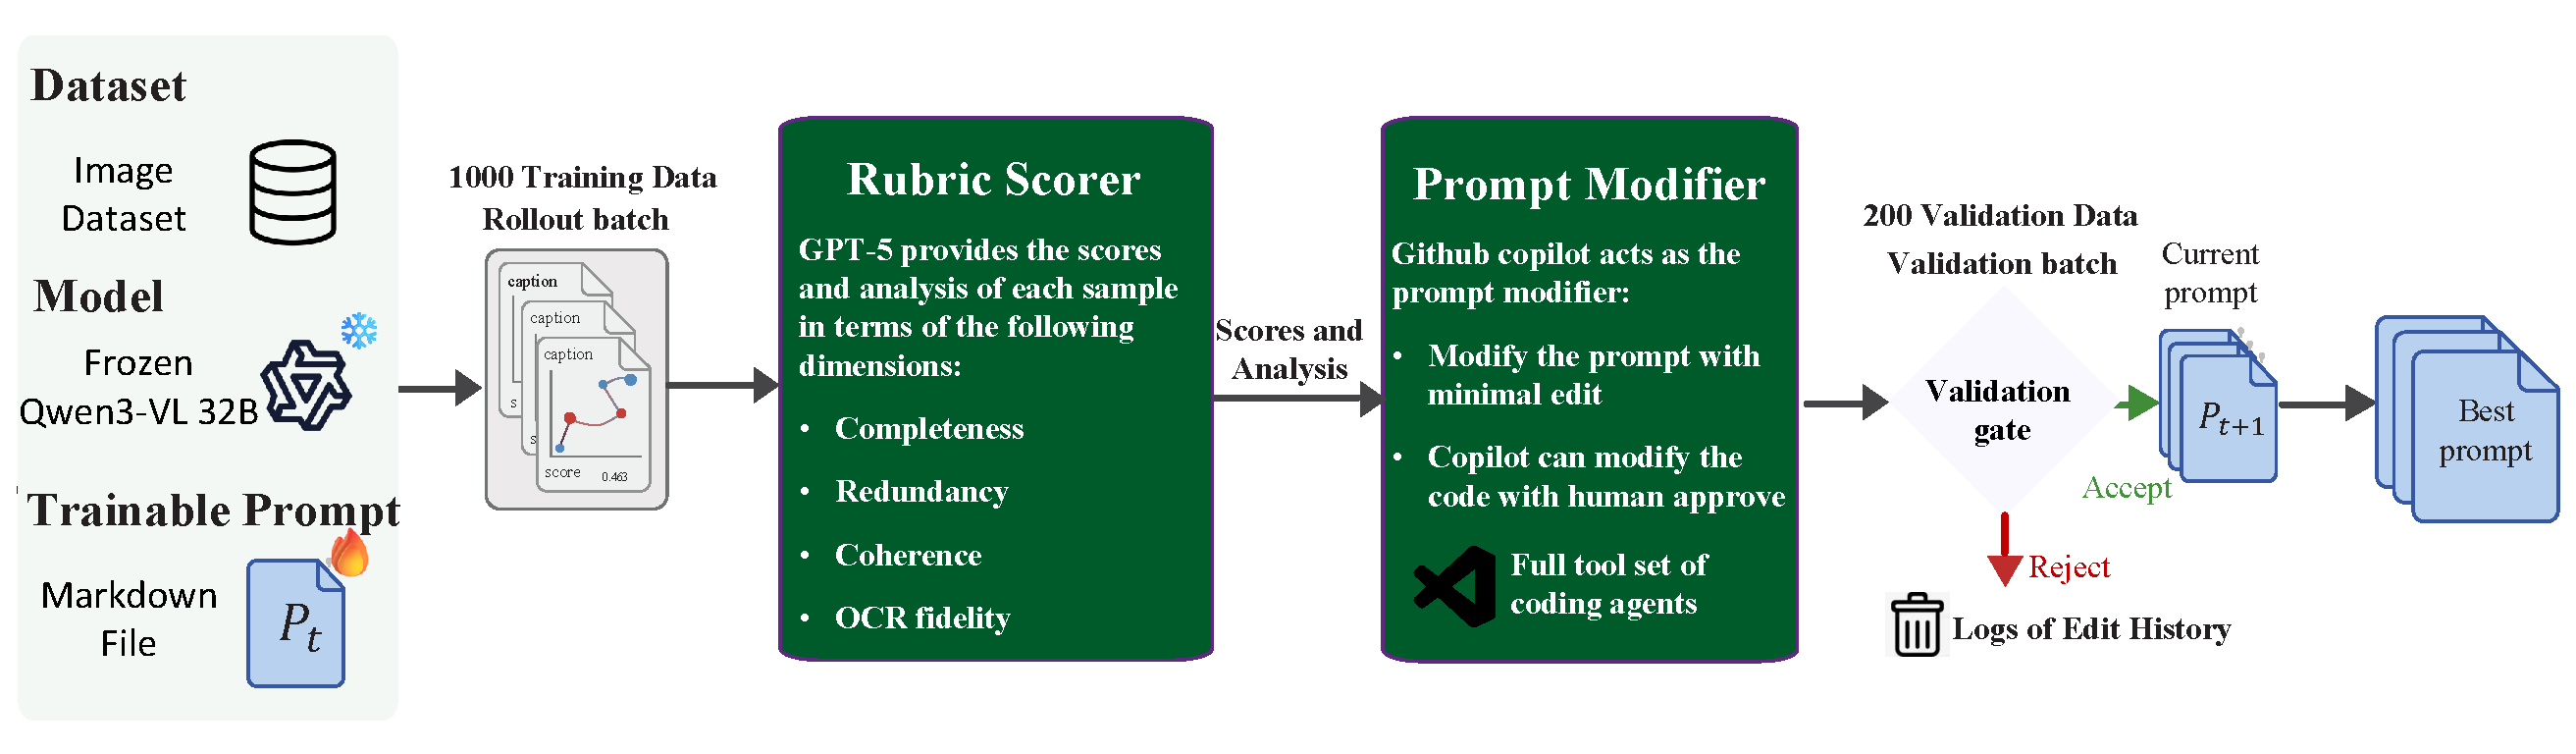
\includegraphics[width=\textwidth]{figures/Caption.pdf} 
    \caption{\textbf{Iterative prompt-optimization pipeline for image recaptioning.} A frozen Qwen3-VL-32B generates captions for a rollout batch, which are evaluated by a GPT-5 Rubric Scorer for completeness, redundancy, coherence, and OCR fidelity. GitHub Copilot then proposes minimal prompt or code revisions, which are evaluated on a held-out validation batch and accepted only after human review.}
    \label{fig:prompt_optimization_pipeline}
\end{figure}



We initialize the optimization process with a rollout batch of 1,000 training images uniformly sampled from ten representative visual domains, with 100 images from each domain. These domains cover diverse content distributions, including natural scenes, people, objects, documents, charts, rendered text, artworks, screenshots, and other visually structured content. Initial captions are generated using the baseline LLaVA-OneVision-1.5 recaptioning prompt~\cite{li2024llavaonevision15}.


For each optimization iteration, a rubric-scoring agent powered by GPT-5 evaluates the generated captions along four dimensions:
\begin{itemize}
    \item \textbf{Completeness:} whether the caption covers the major objects, attributes, actions, spatial relationships, and contextual information visible in the image;
    \item \textbf{Redundancy:} whether the caption contains repeated, verbose, or semantically duplicated descriptions;
    \item \textbf{Coherence:} whether the caption is logically organized, grammatically consistent, and easy to follow;
    \item \textbf{OCR fidelity:} whether visible text is correctly transcribed, preserved in its original language, and associated with the appropriate visual region or document structure.
\end{itemize}

Based on the scores and diagnostic analysis, a prompt-refinement agent, implemented via GitHub Copilot equipped with a full toolset of coding agents, proposes modifications to the current prompt ($P_t$). Guided by the principle of making minimal edits, Copilot refines the prompt within a Markdown file. The proposed prompt is then evaluated through a validation gate using a separate validation batch of 200 images. A human reviewer oversees this process to approve or reject the modification. Revisions that fail the validation gate are rejected and archived into the logs of edit history, while approved revisions are accepted as the new baseline prompt ($P_{t+1}$) for the next iteration. We repeat this evaluate--refine--verify cycle for ten iterations, yielding a final prompt that balances visual coverage, language conciseness, structural coherence, and OCR preservation.

The optimized system prompt is then used for large-scale image captioning. As illustrated in \cref{subsec:caption_prompt_ablation}, captions generated with the optimized prompt consistently improve performance across OCR, document, chart, perception, and general visual-reasoning benchmarks. The complete recaptioning system prompt is provided in Appendix~\ref{app:caption_prompt}.

\paragraph{Image instruction data.}
In addition to dense image captions, we collect approximately 54M image-instruction samples. The filtered mixture contains approximately 44.3M samples derived from LLaVA-OneVision-1.5~\citep{li2024llavaonevision15} and FineVision~\citep{finevision25m}, 6.0M samples from OpenBee~\citep{zhang2026beehighqualitycorpusfullstack}, and 4.6M spatial and GUI instruction samples from LLaVA-OneVision-2~\citep{llavaonevision2}.
The mixture covers general visual question answering, OCR, documents, charts, STEM and mathematical reasoning, multi-image understanding, spatial grounding, GUI understanding, and structured multimodal reasoning. The spatial subset emphasizes object size, count, relative direction, distance, depth, and appearance order, while the GUI subset covers interface-element recognition, localization, and action-oriented reasoning.
During later video stages, subsets of these samples are interleaved with video-caption and video-instruction data. This mixed training preserves image reasoning and instruction-following capabilities as the temporal context is progressively extended.


\subsubsection{Video Data}
\label{sec:video_data}
Our video-caption corpus~\citep{llavaonevision2} contains approximately \textbf{7.95M unique samples}: 4.2M videos of up to 30 seconds, 2.7M videos spanning 30--60 seconds, 0.7M videos spanning 60--180 seconds, and 350K videos of approximately 10--15 minutes. For the 350K long-video subset, we divide each video into non-overlapping segments and estimate content density using codec-stream bit counts, retaining the segment with the highest bit count as the most visually dynamic interval. This subset is initially processed through standard frame sampling and later revisited using codec-stream tokenization, but is counted only once in the unique-sample total. We additionally incorporate LLaVA-Video-178K~\citep{zhang2025llavavideovideoinstructiontuning}, TimeLens~\citep{zhang2026timelensrethinkingvideotemporal}, VideoChat-Flash-Training-Data~\citep{videochatflash2025}, Molmo2-VideoTrack, and Molmo2-VideoPoint~\citep{clark2026molmo2} for video question answering, temporal grounding, tracking, point-based localization, and spatio-temporal reasoning.

\paragraph{Duration-stratified video captions.}
The 4.2M short videos are sampled at 1 fps with at most 30 frames and primarily describe local actions, brief interactions, and object-state changes. The 30--60-second and 60--180-second subsets use up to 60 and 90 frames, respectively, providing supervision for multi-step activities, scene transitions, event ordering, and longer action sequences. The 10--15-minute subset initially uses up to 384 sampled frames and captures long-range event progression, repeated actions, scene continuity, and cross-segment dependencies.
Caption granularity is adapted to video duration. Short clips receive compact, action-dense descriptions, whereas longer videos use segment-level captions with explicit temporal progression and cross-segment references. This supervision teaches the model how visual states evolve over time rather than treating a video as an unordered collection of frames.

\paragraph{Frame-sampled and codec-stream representations.}
All 7.95M video-caption samples are introduced through conventional frame sampling during the early and intermediate training stages. For codec-native adaptation, the 350K long-video subset is converted into temporally ordered codec windows using the patchifier in Fig.~\ref{fig:magevit_framework}. Anchor-frame patches are retained densely, whereas predicted frames contribute only patches selected by codec-derived motion and residual importance. We use configurations of up to 384 and 768 frames.
This conversion preserves the original caption supervision while changing the visual observation interface. Codec-stream tokenization allocates tokens according to spatio-temporal variation rather than assigning a dense patch grid to every sampled frame, enabling denser temporal coverage under a comparable visual-token budget.

\subsubsection{Streaming Event Data}
\label{sec:streaming_event_data}

We construct streaming supervision from our 180-second caption corpus and existing timestamped datasets, including MatchTime~\citep{rao2024matchtimeautomaticsoccergame}, LiveCC~\citep{chen2025livecclearningvideollm}, and StreamingVLM~\citep{xu2026streamingvlmrealtimeunderstandinginfinite}. All sources are converted into a unified real-time \emph{speak}/\emph{silent} format.


\begin{figure*}[t]
    \centering
    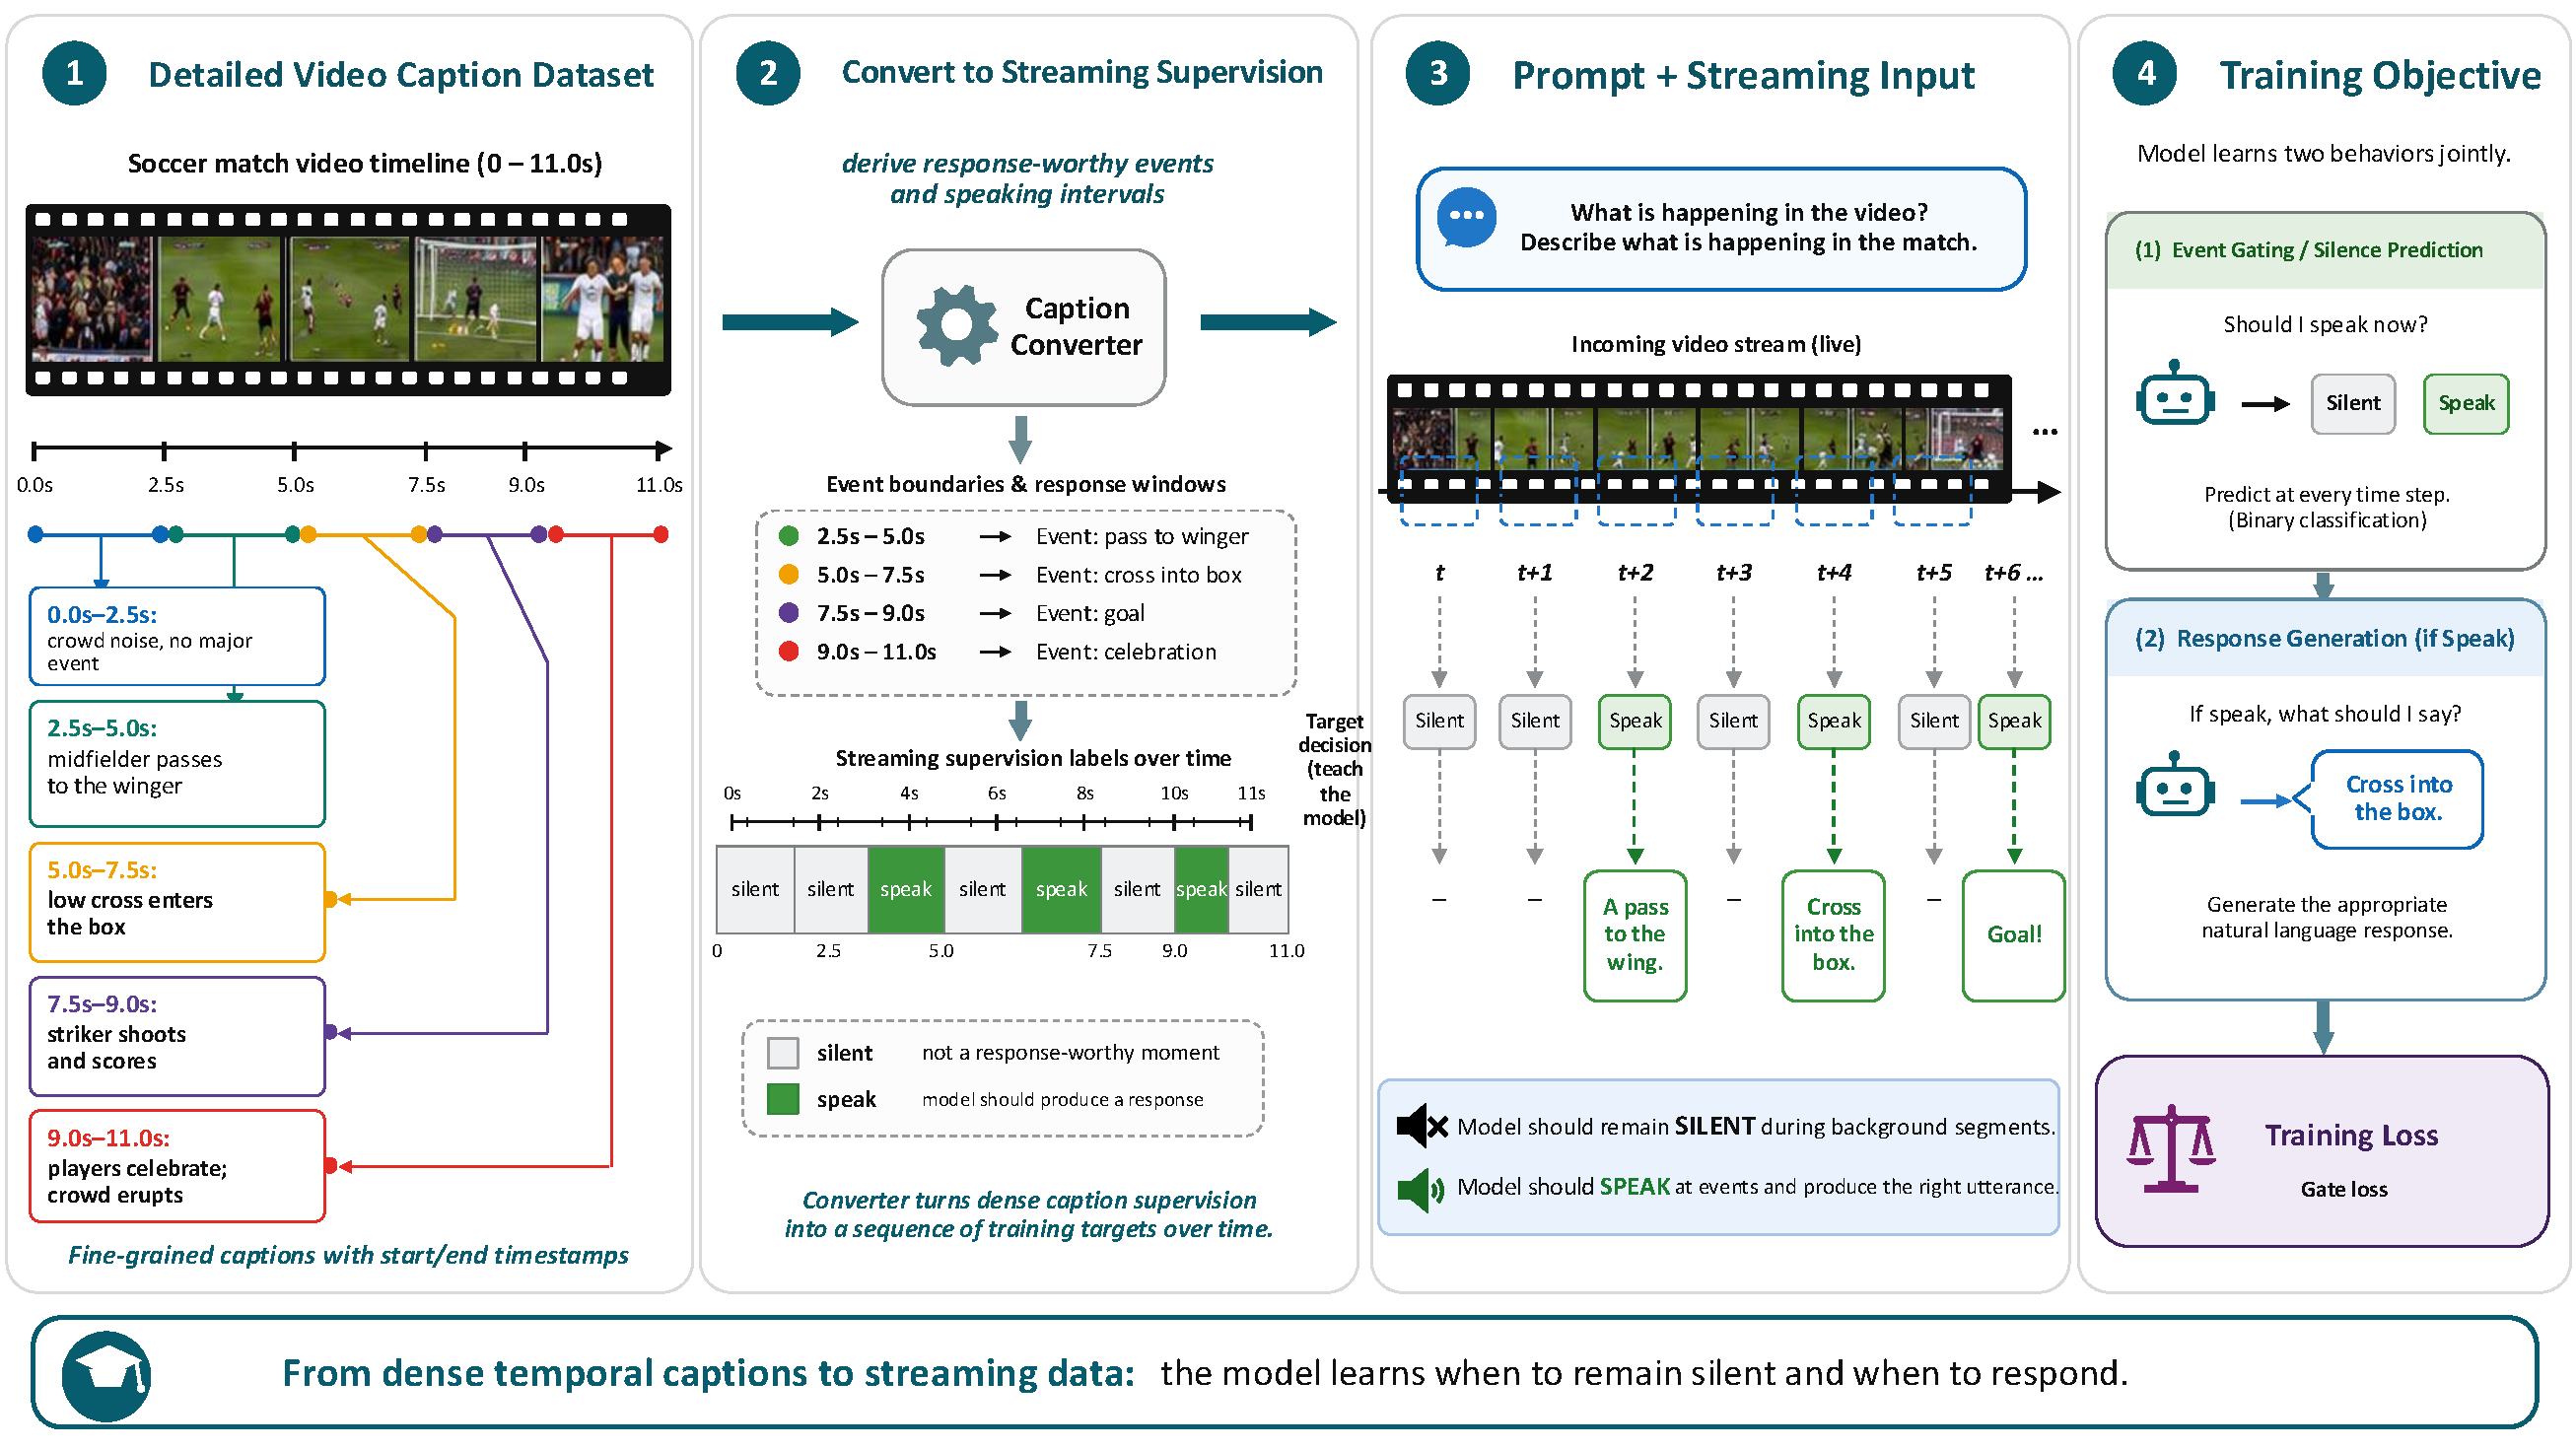
\includegraphics[width=\textwidth]{figures/Streaming_Data_V6.pdf}
    \caption{\textbf{Constructing proactive streaming supervision from timestamped video captions.} Timestamped captions are converted into gate and response targets over causal video prefixes. At each caption start timestamp, the target is \emph{speak} and the corresponding caption provides the response; all other candidate timestamps are labeled \emph{silent}. This supervision teaches the model when to remain silent and when to generate an event-conditioned response.}
    \label{fig:streaming_data}
\end{figure*}


Our streaming corpus contains \textbf{3.3M training samples}: 2.8M samples converted from our 180-second caption data and 0.5M samples derived from existing timestamped streaming datasets. Each sample consists of a causal video prefix, a binary \emph{speak}/\emph{silent} target, and (for positive instances) a corresponding language response. All sources are normalized into the same real-time annotation format.



As illustrated in \cref{fig:streaming_data}, an annotated video is represented as
\[
\mathcal{V}=\{(s_j,e_j,c_j)\}_{j=1}^{N},
\]
where $s_j$ and $e_j$ denote the start and end timestamps of the $j$-th segment, and $c_j$ describes the corresponding event, action, or speech. Following the event-gated formulation of StreamMind~\citep{ding2025streammindunlockingframerate}, a caption converter transforms these timestamped annotations into real-time gate and response targets.

For each caption $(s_j,e_j,c_j)$, the start timestamp $s_j$ is assigned a positive \emph{speak} label and paired with $c_j$ as the target response. Candidate timestamps that do not begin a caption receive a negative \emph{silent} label. Applying this conversion to the 180-second caption corpus produces 2,801,360 real-time training samples.

All examples satisfy a \emph{no-future-frame} constraint: the gate decision and target response depend only on observations available up to the current timestamp. Applying the same conversion to the existing timestamped datasets produces the remaining 543,943 samples and increases the diversity of events, response styles, and interaction timings.

\subsubsection{Data Curation and Balancing}
\label{sec:data_curation}
All data mixtures are filtered for corrupted files, unsafe content, low-quality samples, and near-duplicates. For caption data, we additionally remove captions that are too short to provide meaningful visual grounding, captions whose timestamps are inconsistent with the video duration, repeated or near-duplicate temporal descriptions, and samples flagged by caption--video consistency checks. For streaming supervision, we balance the \emph{speak}/\emph{silent} labels produced by the caption converter by subsampling redundant silent timestamps.

We balance the corpus along two additional axes. Domain balancing upweights regimes that are underrepresented in web data but important for evaluation and deployment, including OCR, documents, charts, STEM and mathematics, spatial reasoning, temporal grounding, and streaming events. Duration balancing controls the proportions of short, medium, long, and ultra-long videos at each training stage. Overall, the early stages inherit the open-data family of LLaVA-OneVision-style training, but place greater emphasis on scaled dense image captions, temporally precise video captions, codec-stream supervision, and calibrated cognition-gate targets.



% We then balance the corpus along two axes. Domain balancing upweights regimes that are
% under-represented in web data but important for evaluation and deployment, including OCR,
% documents, charts, STEM/math, spatial reasoning, temporal grounding, and streaming events. Duration
% balancing controls the ratio of short, medium, long, and ultra-long videos at each training stage.
% Overall, the early stages inherit the open-data family of LLaVA-OneVision-style training, but the
% emphasis is shifted toward scaled dense image captions, temporally precise video captions,
% codec-stream supervision, and well-calibrated visual-gate targets for \magevl's streaming
% objective.

\subsection{Progressive Training Curriculum}
\label{sec:magevl_training}

\magevl is trained through a progressive five-stage supervised curriculum. The five stages successively establish visual-language grounding, instruction following, temporal-context extension, codec-native long-context adaptation, and proactive streaming alignment. Together, they produce a single unified model that supports image understanding, offline video reasoning, and proactive interaction over continuous video streams. 

\paragraph{Stage 1: Multimodal alignment via captions.}
Stage~1 uses approximately 350M dense image captions and 4.2M short-video captions~\citep{llavaonevision2}. Dense image captions provide the dominant supervision, forcing the model to associate \magevit tokens with objects, attributes, OCR text, charts, documents, spatial relationships, and global scene context. Fine-grained short-video captions are included from the beginning so that the model encounters motion and state changes before the long-video curriculum. Unlike a projector-only alignment stage, this warm-up directly trains the model as a caption-capable multimodal language model.


% Stage~1 uses approximately 350M dense image captions and 4.2M short-video captions~\citep{llavaonevision2}, together with a lightweight general SFT mixture. Dense image captions form
% the dominant supervision source, because they force the model to associate \magevit tokens with
% objects, attributes, OCR text, charts, documents, spatial relations, and global scene context. We
% also include fine-grained short-video captions from the beginning, so the model is exposed to motion
% and state changes before any long-video curriculum. In contrast to a
% pure projector-alignment stage, this warm-up already trains the model as a caption-capable
% multimodal language model, with image captions providing the majority of optimization signal.

\paragraph{Stage 2: Instruction tuning and short temporal grounding.}
Stage~2 uses approximately 54M image-instruction samples from LLaVA-OneVision-1.5~\citep{li2024llavaonevision15}, FineVision~\citep{finevision25m}, OpenBee~\citep{zhang2026beehighqualitycorpusfullstack}, and LLaVA-OneVision-2 spatial and GUI data~\citep{llavaonevision2}, together with 3.4M video captions spanning 30--180 seconds~\citep{llavaonevision2}. We increase the weight of multimodal instruction data, particularly OCR, document QA, chart reasoning, STEM and mathematics, multi-image reasoning, spatial grounding, and GUI understanding. Short-video captions and instructions remain active to provide local temporal grounding for actions and object-state transitions. Generic language-only or weakly visual SFT is assigned a low weight so that it does not dominate the visual grounding acquired in Stage~1. This stage transforms the model from a visual describer into a general multimodal assistant while retaining caption supervision as regularization.


% Stage~2 uses approximately 54M image-instruction samples from LLaVA-OneVision-1.5~\citep{li2024llavaonevision15}, FineVision~\citep{finevision25m}, OpenBee~\citep{zhang2026beehighqualitycorpusfullstack}, and LLaVA-OneVision-2 spatial/GUI data~\citep{llavaonevision2}, together with 3.4M video captions spanning 30--180 seconds. We increase the weight
% of image and multimodal SFT data, especially OCR, document QA, chart reasoning, STEM/math,
% multi-image reasoning, spatial grounding, and GUI/screenshot understanding. At the same time, short
% video captions and short video instructions remain active, providing local temporal grounding for
% actions and object-state transitions. Generic language-only or weakly visual SFT is kept at a low
% weight; it is useful for response style but should not dominate the visual grounding learned in
% Stage~1. This stage turns the model from a strong visual describer into a general multimodal
% assistant while preserving caption supervision as regularization.

\paragraph{Stage 3: Temporal-horizon expansion.}
Stage~3 retains 20M Stage-2 image-instruction samples and introduces medium- and long-video data from LLaVA-Video~\citep{zhang2025llavavideovideoinstructiontuning}, TimeLens~\citep{zhang2026timelensrethinkingvideotemporal}, VideoChat-Flash~\citep{videochatflash2025}, Molmo2~\citep{clark2026molmo2}, and our temporally structured captions. These data describe event order, scene transitions, repeated actions, and cross-segment dependencies. The goal is not simply to expose the model to more frames, but to teach it how visual states evolve over minutes and how later events depend on earlier context. Image SFT, spatial data, GUI data, and short-video samples remain in the mixture to preserve static perception and instruction-following capabilities. \textbf{We also employ AI4AI at this stage. Specifically, we employ AI-based diagnostics to pinpoint underperforming or missing capabilities, which are subsequently addressed by targeted human data supplementation. Meanwhile, these diagnostics dynamically guide the selection of the optimal resolution and frame count.}


% Stage~3 retains 20M Stage-2 image-instruction samples and adds medium- and long-video data from LLaVA-Video~\citep{zhang2025llavavideovideoinstructiontuning}, TimeLens~\citep{zhang2026timelensrethinkingvideotemporal}, VideoChat-Flash~\citep{videochatflash2025}, Molmo2~\citep{clark2026molmo2}, and our temporally structured captions, which describe event order, scene transitions, repeated actions,
% and cross-segment references. The goal is not simply to show the model more frames, but to teach it
% how visual states evolve over minutes and how later events depend on earlier context. Image SFT,
% spatial data, GUI data, and short-video samples are still retained in the mixture to prevent the
% longer video objective from eroding static perception and instruction-following abilities.

\paragraph{Stage 4: Codec-native long-context adaptation.}
Stage~4 uses 350K long-video captions, 4M spatial samples~\citep{llavaonevision2}, Molmo2 tracking and pointing data~\citep{clark2026molmo2}, and 40M retained image-instruction samples. After the model has learned to reason over extended temporal contexts, we convert a large fraction of video training into the codec-native representation used at inference time. Captioned videos are represented as rolling token windows containing dense anchor-frame evidence and sparse predicted-frame updates. This stage adapts the language model to the irregular visual sequences produced by \magevit, where token density follows visual change rather than fixed frame slots. Long and ultra-long videos benefit most from this representation because the model can observe more event boundaries under the same visual-token budget. Non-video instruction data remain in the mixture to preserve image, OCR, chart, spatial, and GUI capabilities.


% Stage~4 uses 350K long-video captions and 4M spatial samples~\citep{llavaonevision2}, Molmo2 tracking and pointing data~\citep{clark2026molmo2}, and 40M retained image-instruction samples. After the model has learned to reason over longer temporal contexts, we switch a large fraction of
% video training to the codec-native format used at inference time. Captioned videos are converted
% into rolling token windows containing dense anchor-frame evidence and sparse predicted-frame
% evidence. This stage adapts the LLM to the irregular visual sequence produced by \magevit: token
% density now follows visual change rather than fixed frame slots. Long and ultra-long videos benefit
% most from this representation, since the model can observe more event boundaries under the same
% visual-token budget. Non-video instruction data remains in the background mixture as an anchor for
% static image, OCR, chart, spatial, and GUI capabilities. The resulting
% checkpoint is denoted as \magevlbase.


\paragraph{Stage 5: Proactive streaming alignment via cognition-gate fine-tuning.}
In Stage~5, we introduce a lightweight cognition gate to enable proactive streaming interaction while keeping the base language model completely frozen. For each causal segment, the codec-extraction pipeline packs codec-selected patches into a compact canvas while preserving their original spatio-temporal coordinates. These features are processed by the event-preserving feature extractor (EPFE), whose recurrent state maintains a streaming perception memory $\mathcal{M}_{\mathrm{per}}$ used exclusively by the cognition gate for real-time turn-taking decisions. Crucially, when the gate issues a \emph{speak} decision, we do not employ complex long-range memory for language generation. Instead, the model invokes the frozen base VLM directly using a local sliding window of the most recent $N$ codec-assembled visual segments as input context to execute standard autoregressive response generation. We train the cognition gate on approximately 3.35M streaming samples: 2.8M converted from 180-second captions and 0.54M converted from MatchTime~\citep{rao2024matchtimeautomaticsoccergame}, LiveCC~\citep{chen2025livecclearningvideollm}, and StreamingVLM~\citep{xu2026streamingvlmrealtimeunderstandinginfinite}, as described in \cref{sec:streaming_event_data}.

Throughout this stage, the visual backbone, EPFE, and language model remain strictly frozen, and we solely fine-tune the cognition gate. At every candidate timestamp, the gate autoregressively evaluates the accumulated streaming memory $\mathcal{M}_{\mathrm{per}}$ and predicts one of two tokens: \emph{silent} or \emph{speak}. Caption start timestamps provide speak targets, while all other timestamps serve as silent targets. To address the inherent sparsity of speak events, we optimize a class-weighted token cross-entropy loss:
\[
\mathcal{L}_{\mathrm{gate}}
=
-\sum_t w_{g_t}\log p(g_t \mid g_{<t}, \mathcal{M}_{\mathrm{per}}),
\qquad g_t\in\{\text{silent},\text{speak}\}.
\]
When $g_t=\text{speak}$, the recent $N$-segment codec visual canvas is passed directly to the frozen language model for autoregressive generation. Restricting optimization to the cognition gate adds proactive response timing while preserving the image and video understanding capabilities acquired during the preceding stages.